\documentclass[10pt]{beamer}
\usepackage[spanish]{babel}
\usepackage{csquotes}
\usepackage[T1]{fontenc}

\setbeameroption{hide notes} % Only slides
%\setbeameroption{show only notes} % Only notes
%\setbeameroption{show notes on second screen=bottom} % Both

\usepackage{graphicx}
\usepackage{colortbl}

\usetheme{moloch}
\molochset{block=fill}

\setbeamertemplate{page number in head/foot}[appendixframenumber]
\setbeamertemplate{section in toc}[sections numbered]

\usepackage{plex-serif}
\usepackage{plex-sans}
\usepackage{plex-mono}

% Unidades
\usepackage[locale=DE]{siunitx}

% Bibliografia
\usepackage[style=apa, backend=biber]{biblatex}
\renewrobustcmd*{\mkbibfootnote}[1]{\footnote[frame]{#1}}
\setbeamertemplate{footnote}{% Footnote spacing fix for double digits
  \hspace{2pt}%
  \makebox[1em][l]{\insertfootnotemark}%
  \insertfootnotetext\par%
}
\addbibresource{bachelor-thesis/referencias.bib}

% Links
\usepackage{hyperref}
\hypersetup{colorlinks=true,linkcolor=black,citecolor=.,urlcolor=blue}

\title{Sistema de Monitoreo y Alerta Temprana basado en IA para Áreas Protegidas}
\subtitle{Proyecto Final Integrador - Ingeniería en Computación}
\author{Fabrizio Contigiani - Gabriel Da Silva Schmies}
\institute{Tutor: Dr. Ing. Sergio Moya} % institute already in titlegraphic
\date{23 de junio de 2026}
\titlegraphic{
\includegraphics[height=1.5cm]{img/logo_unam.png}\hfill
\includegraphics[height=1.5cm]{img/logo_fio.png}}
% Paquetes añadidos para diagramas vectoriales nativos (TikZ/PGFPlots)
\usepackage{tikz}
\usetikzlibrary{shapes.geometric, shapes.symbols, arrows.meta, positioning, fit, backgrounds, calc, babel}
\usepackage{pgfplots}
\pgfplotsset{compat=1.18}
\usepackage{subcaption}
\usepackage{tabularray}

\begin{document}


\maketitle

\begin{frame}{Índice}
  \tableofcontents
  \note{
    Presentar brevemente la estructura de la exposición.
  }
\end{frame}

% ==============================================================================
% Sección 1: Motivación
% ==============================================================================
\section{Motivación}

\begin{frame}[plain]
  \begin{tikzpicture}[remember picture, overlay]
    \node[anchor=center] at (current page.center) {
      \includegraphics[height=\paperheight,keepaspectratio]{img/talking.png}
    };
  \end{tikzpicture}
\end{frame}

\begin{frame}[standout]
¿Misiones?
\end{frame}

\begin{frame}[plain]
  \begin{tikzpicture}[remember picture, overlay]
    \node[anchor=center] at (current page.center) {
      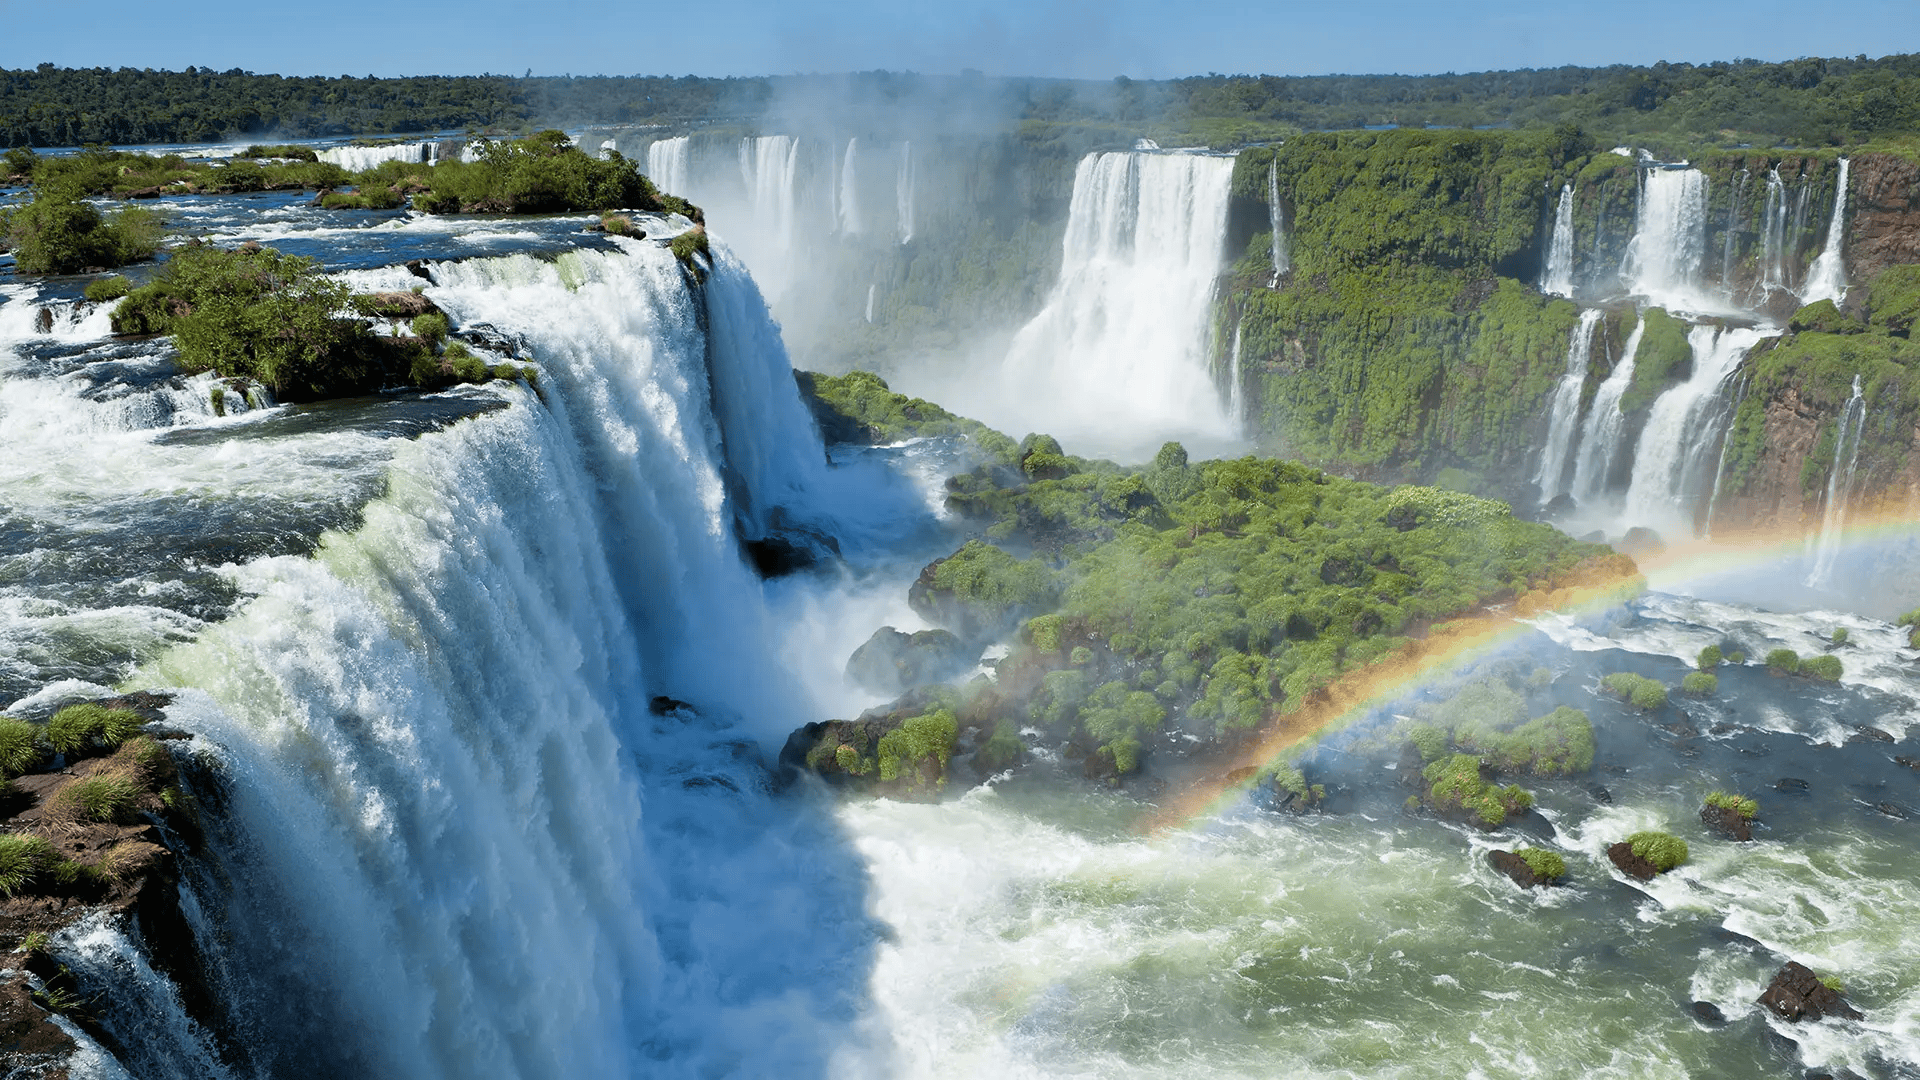
\includegraphics[height=\paperheight,keepaspectratio]{img/iguazu-falls.png}
    };
  \end{tikzpicture}
\end{frame}

\begin{frame}[plain]
  \begin{tikzpicture}[remember picture, overlay]
    \node[anchor=center] at (current page.center) {
      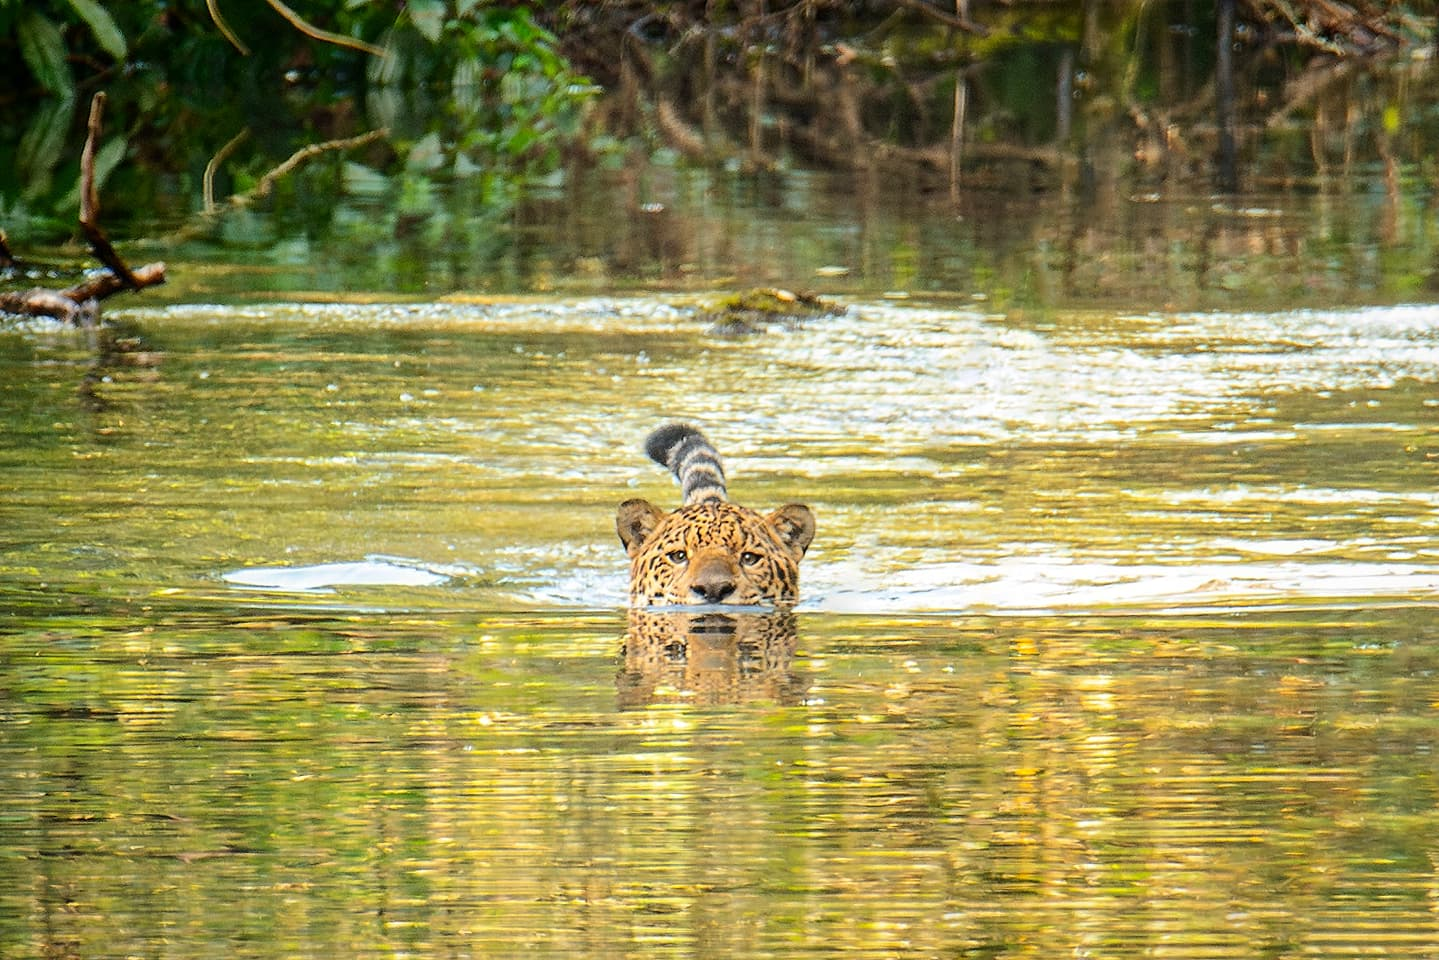
\includegraphics[height=\paperheight,keepaspectratio]{img/yag1.jpg}
    };
  \end{tikzpicture}
\end{frame}

\begin{frame}[plain]
  \begin{tikzpicture}[remember picture, overlay]
    \node[anchor=center] at (current page.center) {
      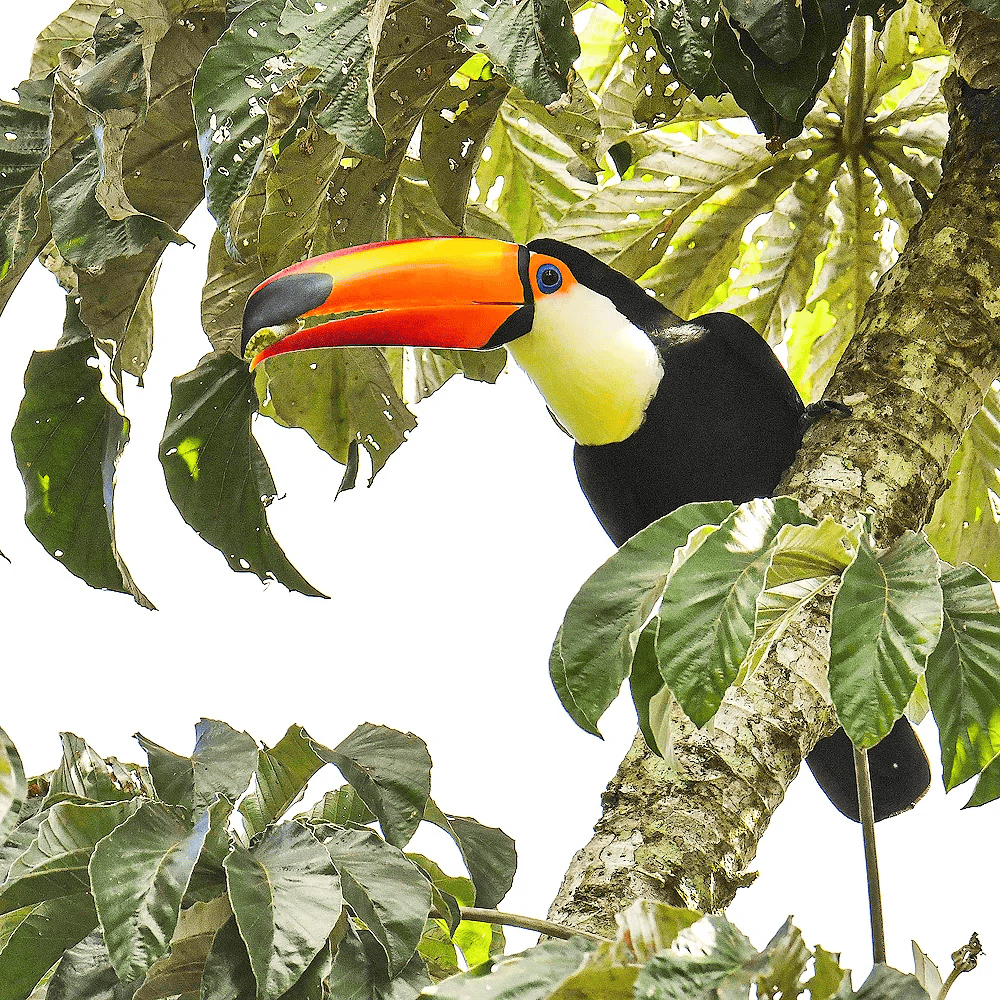
\includegraphics[height=\paperheight,keepaspectratio]{img/tucan.png}
    };
  \end{tikzpicture}
\end{frame}

\begin{frame}[standout]
Más que eso...
\end{frame}

\begin{frame}[plain]
  \begin{tikzpicture}[remember picture, overlay]
    \node[anchor=center] at (current page.center) {
      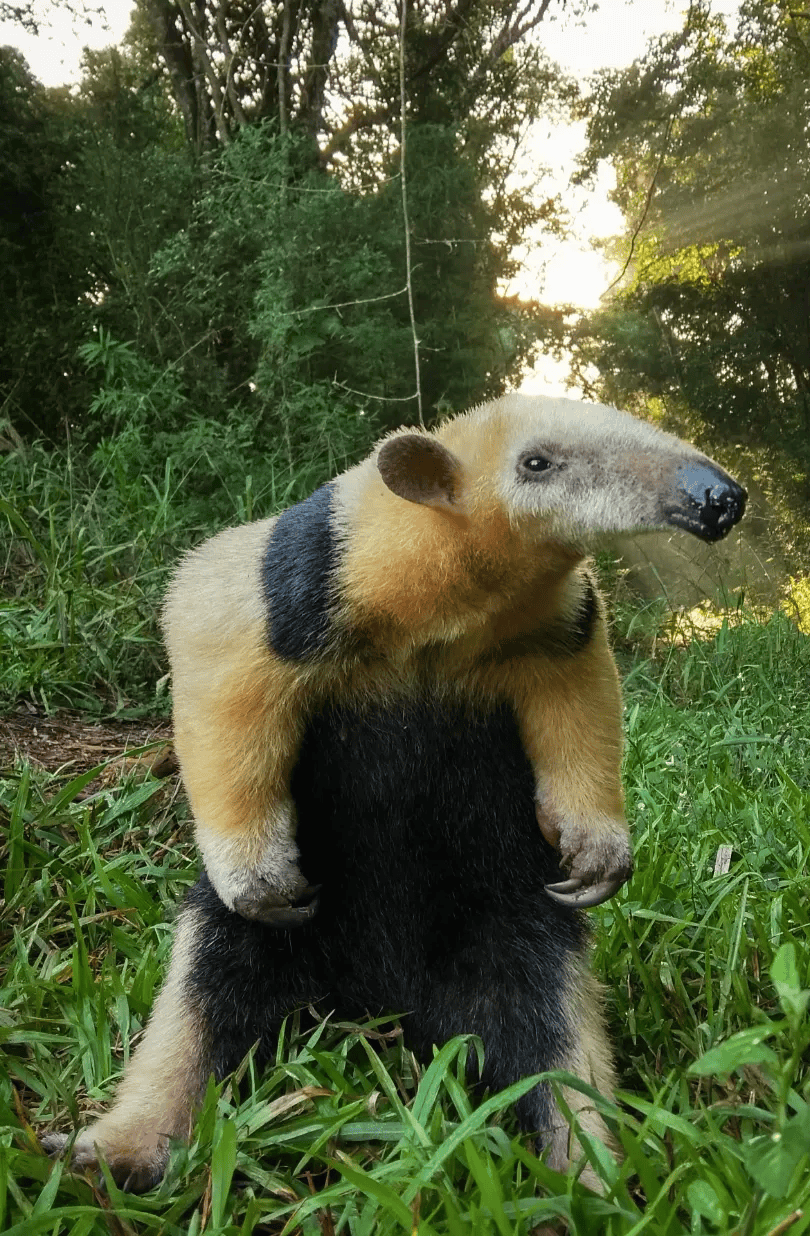
\includegraphics[height=\paperheight,keepaspectratio]{img/oso.png}
      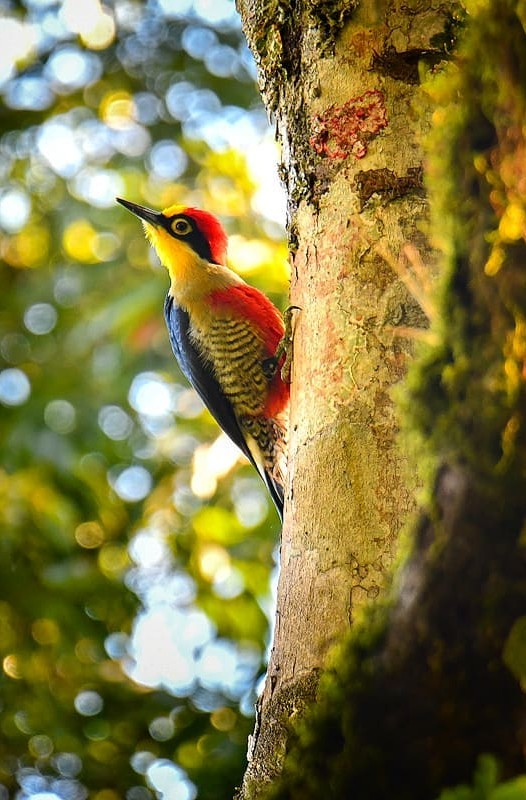
\includegraphics[height=\paperheight,keepaspectratio]{img/misiones5.jpg}
    };
  \end{tikzpicture}
\end{frame}

\begin{frame}[plain]
  \begin{tikzpicture}[remember picture, overlay]
    \node[anchor=center] at (current page.center) {
      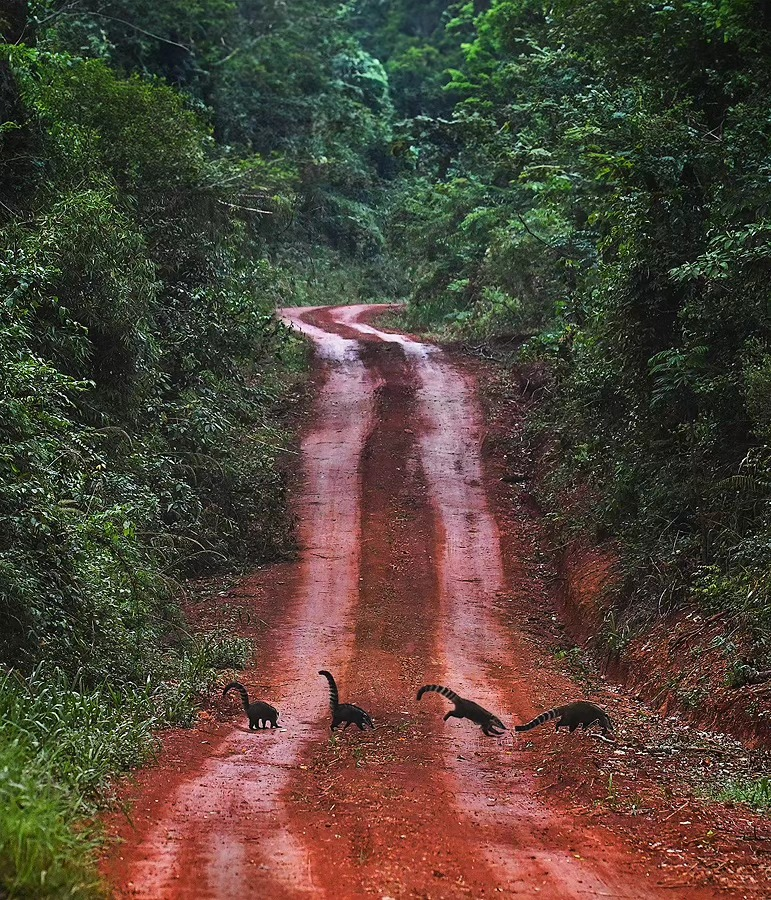
\includegraphics[height=\paperheight,keepaspectratio]{img/misiones3.jpg}
      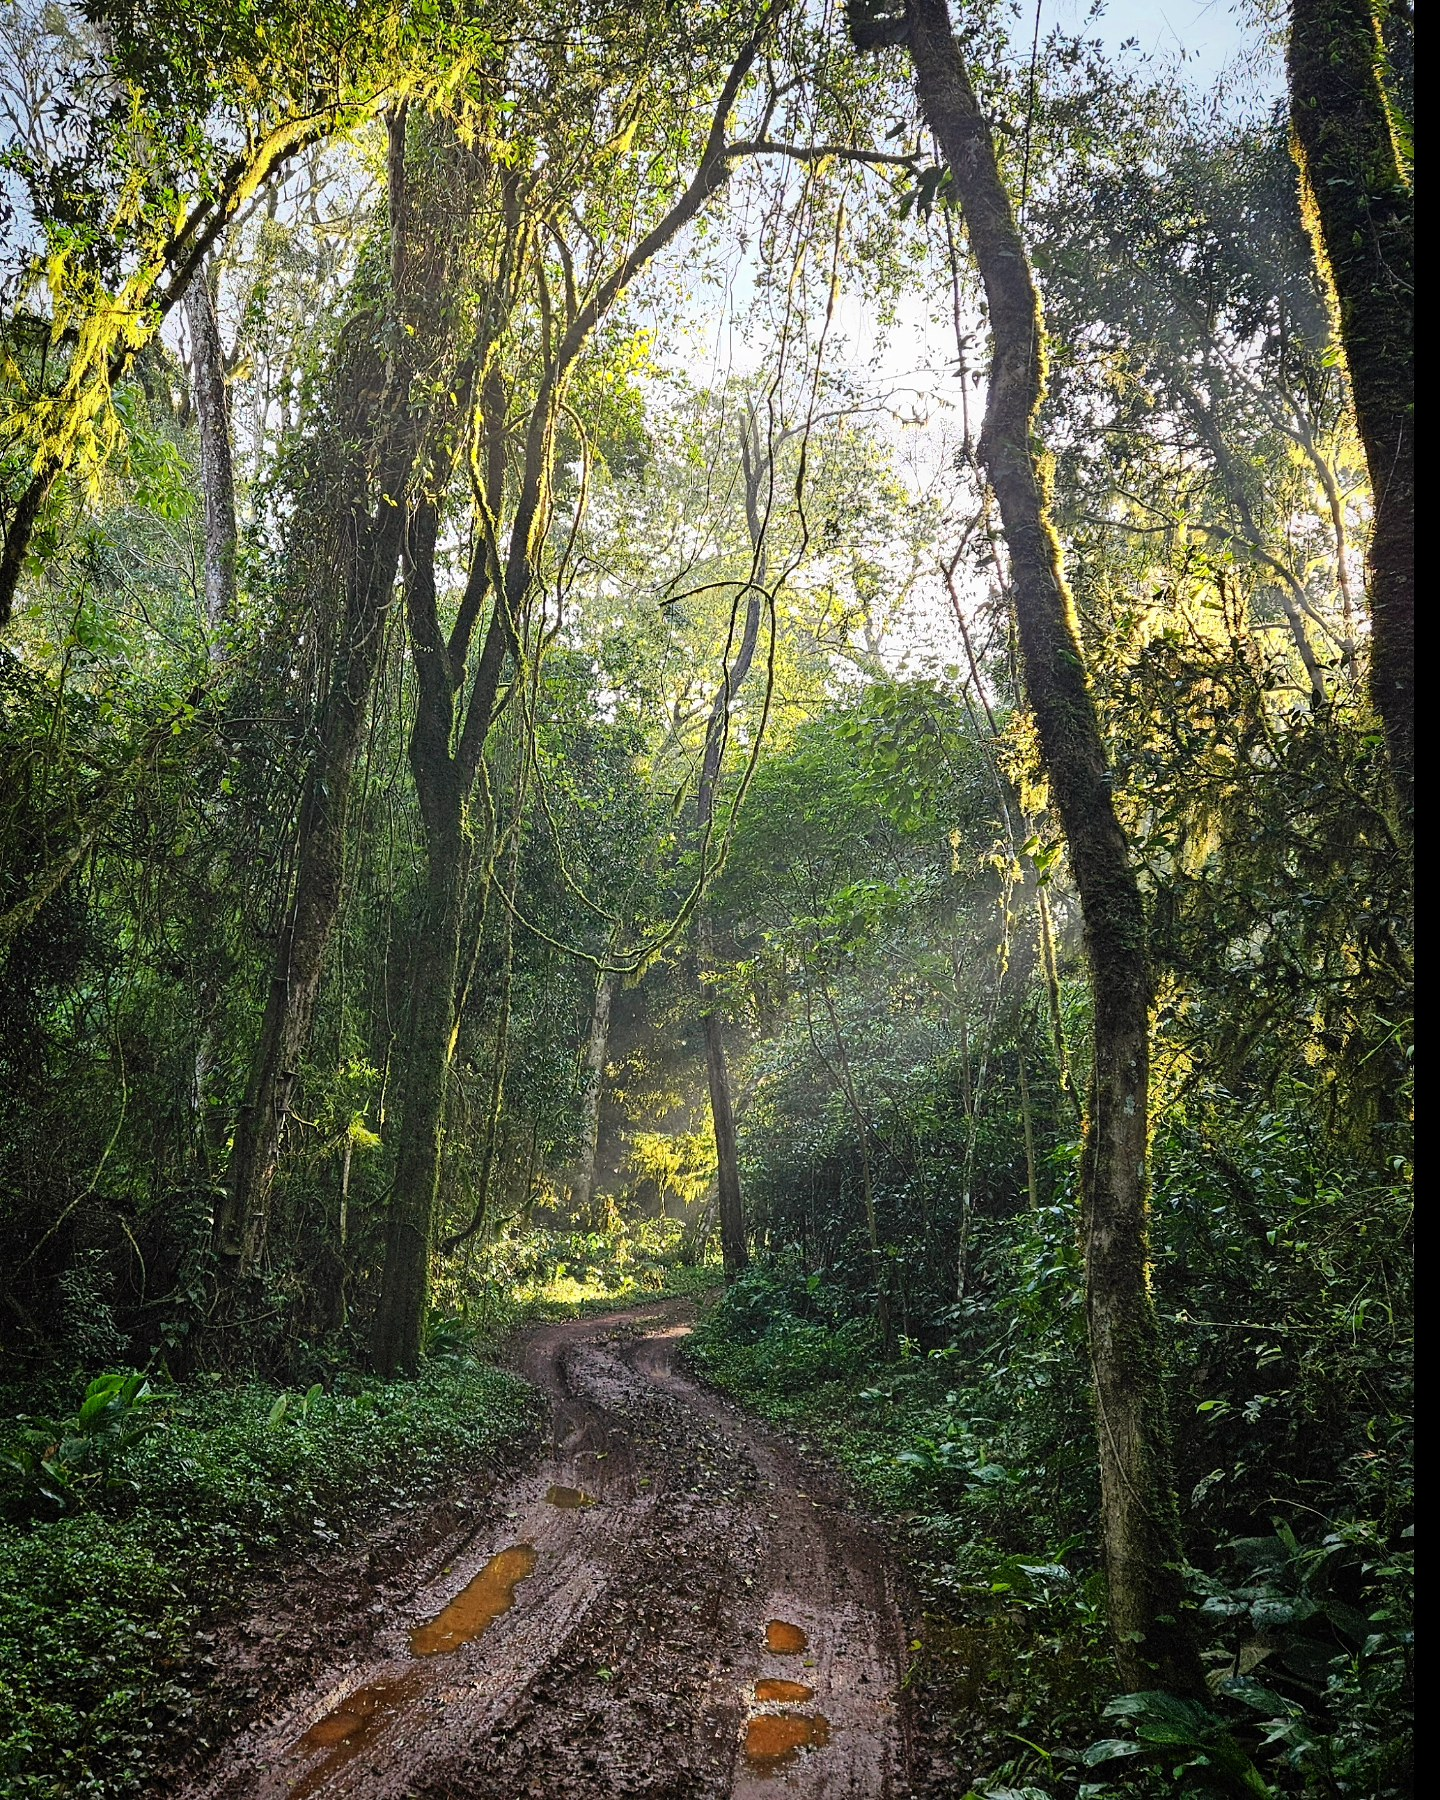
\includegraphics[height=\paperheight,keepaspectratio]{img/misiones2.jpg}
    };
  \end{tikzpicture}
\end{frame}

\begin{frame}[plain]
  \begin{tikzpicture}[remember picture, overlay]
    \node[anchor=center] at (current page.center) {
      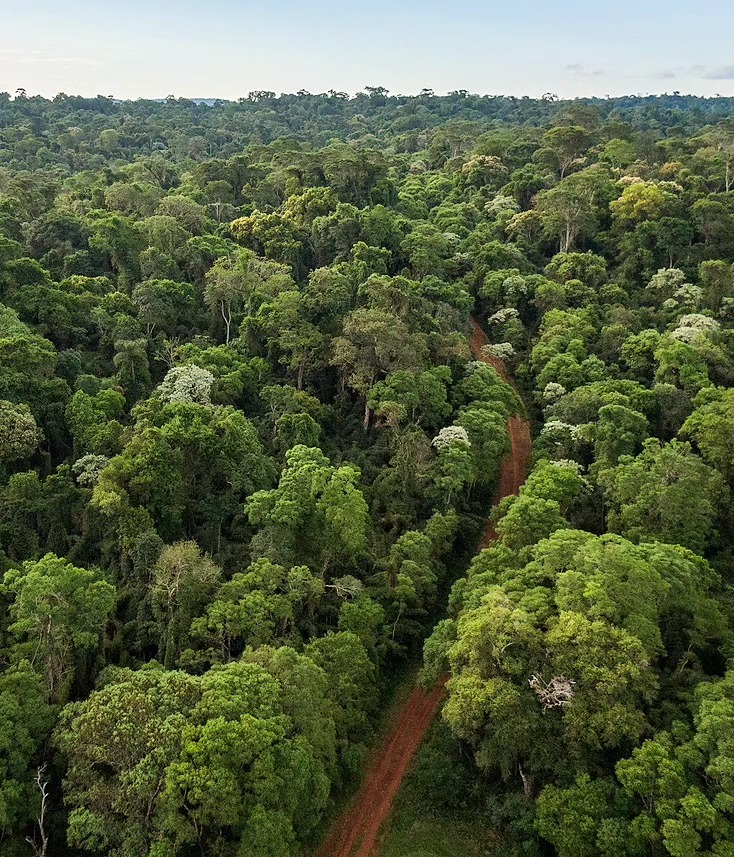
\includegraphics[height=\paperheight,keepaspectratio]{img/misiones4.jpg}
      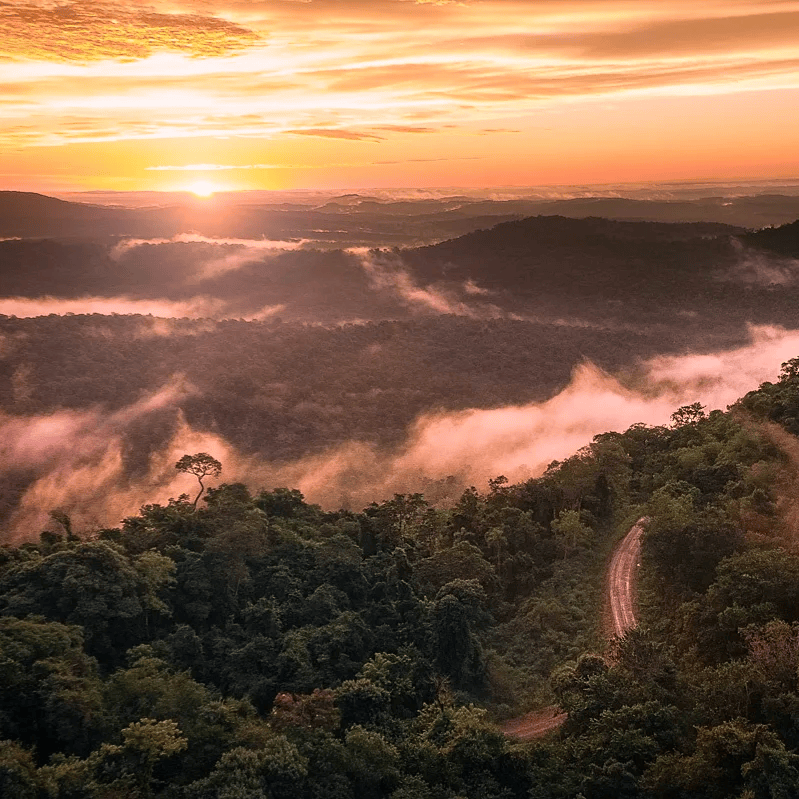
\includegraphics[height=\paperheight,keepaspectratio]{img/misiones6.png}
    };
  \end{tikzpicture}
\end{frame}

\begin{frame}[standout]
Ejercicio
\end{frame}

\begin{frame}[plain]
  \begin{tikzpicture}[remember picture, overlay]
    \node[anchor=center] at (current page.center) {
      \includegraphics[height=\paperheight,keepaspectratio]{img/map1_cropped.pdf}
    };
  \end{tikzpicture}
\end{frame}

\begin{frame}[plain]
  \begin{tikzpicture}[remember picture, overlay]
    \node[anchor=center] at (current page.center) {
      \includegraphics[height=\paperheight,keepaspectratio]{img/map2_cropped.pdf}
    };
  \end{tikzpicture}
\end{frame}

\begin{frame}[plain]
  \begin{tikzpicture}[remember picture, overlay]
    \node[anchor=center] at (current page.center) {
      \includegraphics[height=\paperheight,keepaspectratio]{img/map3_cropped.pdf}
    };
  \end{tikzpicture}
\end{frame}

\begin{frame}[plain]
  \begin{tikzpicture}[remember picture, overlay]
    \node[anchor=center] at (current page.center) {
      \includegraphics[height=\paperheight,keepaspectratio]{img/map4_cropped.pdf}
    };
  \end{tikzpicture}
\end{frame}

\begin{frame}[plain]
  \begin{tikzpicture}[remember picture, overlay]
    \node[anchor=center] at (current page.center) {
      \includegraphics[height=\paperheight,keepaspectratio]{img/map5_cropped.pdf}
    };
  \end{tikzpicture}
\end{frame}

\section*{Misiones en números}

\begin{frame}{El Bosque Atlántico}
  \begin{columns}
    \begin{column}{0.5\textwidth}
      \textbf{El marco ecológico global}
      \begin{itemize}
        \item Originalmente: \num{1.3} millones de \unit{\km\squared} \footcite{ribeiro2009atlantic}
        \item Brasil (\qty{92}{\percent}), Paraguay (\qty{6}{\percent}), Argentina (\qty{2}{\percent})
        \item Hoy: solo \qtyrange{12}{17}{\percent} de su extensión original
        \item Uno de los \textbf{hotspots de biodiversidad} más amenazados del planeta \footcite{wwf2024atlantic}
      \end{itemize}
    \end{column}
    \begin{column}{0.5\textwidth}
      \centering
      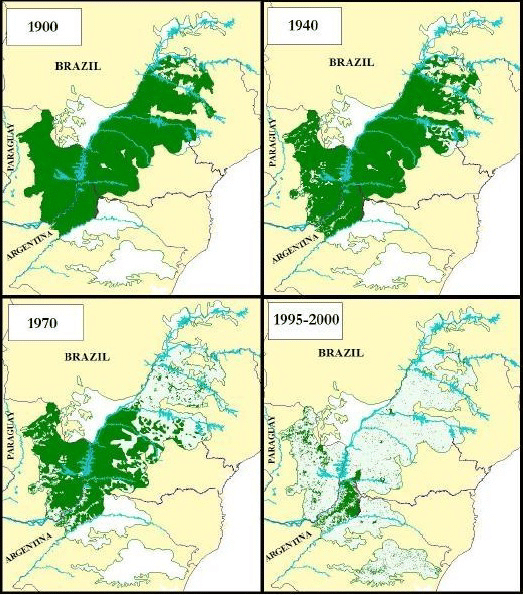
\includegraphics[width=0.95\textwidth]{img/bosque_altantico.png}
      
      \vspace{0.2em}
      {\tiny Fuente: \href{https://www.researchgate.net/figure/Figura-8-Proceso-de-deforestacion-del-Bosque-Atlantico-Alto-Parana-desde-el-ano-1900_fig1_268334207}{ResearchGate (Fig. 8)}}
    \end{column}
  \end{columns}
  \note{
    Arrancamos con el contexto global. El Bosque Atlántico es uno de los hotspots más amenazados del planeta, habiéndose perdido más del 80\% de su cobertura original. Si miran la imagen del proceso de deforestación, el pequeño remanente continuo que sobrevive en la frontera de Argentina es Misiones. Por eso, en la siguiente diapositiva, hacemos foco en esta selva.
  }
\end{frame}

\begin{frame}{La Selva Misionera}
  \begin{columns}
    \begin{column}{0.5\textwidth}
      \begin{itemize}
        \item Mas del \textbf{\qty{50}{\percent} de la biodiversidad} de Argentina \footcite{dibitetti2003yaguarete}
        \item En menos del \qty{0.5}{\percent} del territorio nacional
        \item \num{1.1} millones de hectareas protegidas
        \item \textbf{Corredor Verde de Misiones}
      \end{itemize}

      \vspace{1em}
      Es el \textbf{remanente continuo mas extenso} del Bosque Atlántico en el Cono Sur.
    \end{column}
    \begin{column}{0.5\textwidth}
      \centering
      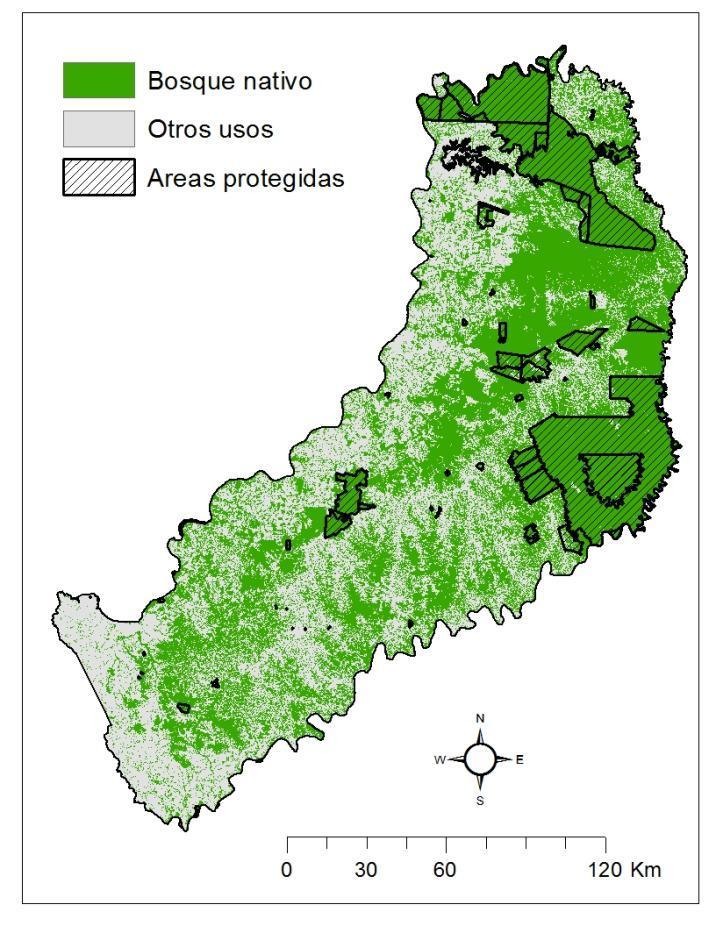
\includegraphics[width=0.95\textwidth]{img/parte_bosque_atlantico_corredor_verde.jpg}
      
      \vspace{0.2em}
      {\tiny Fuente: \href{https://www.researchgate.net/figure/Figura-2-1-Mapa-del-Bosque-Atlantico-de-Misiones-y-las-areas-protegidas-privadas-y_fig2_318351487}{ResearchGate (Fig. 2-1)}}
    \end{column}
  \end{columns}
  \note{
    Hacemos zoom en ese remanente continuo que vimos recién: la Selva Misionera. Concentra más del 50\% de la biodiversidad del país en menos del 0.5\% del territorio. Su gran baluarte es el Corredor Verde de Misiones, que conecta las distintas áreas protegidas públicas y privadas.
  }
\end{frame}

\begin{frame}{Biodiversidad Excepcional}
  \begin{columns}
    \begin{column}{0.55\textwidth}
      \textbf{Concentracion de especies:}
      \begin{itemize}
        \item $\sim$\num{3000} especies de plantas vasculares
        \item \num{554} especies de aves
        \item \num{120} especies de mamiferos
        \item \num{79} reptiles y \num{55} anfibios
      \end{itemize}

      \vspace{0.5em}
      \textbf{Especies emblematicas:}
      \begin{itemize}
        \item Yaguarete (\textit{Panthera onca})
        \item Tapir (\textit{Tapirus terrestris})
        \item Aguila harpia (\textit{Harpia harpyja})
        \item Yacutinga (\textit{Aburria jacutinga})
      \end{itemize}
    \end{column}
    \begin{column}{0.45\textwidth}
      % TODO: Collage de fauna emblematica
      \centering
      \fbox{\parbox{0.9\textwidth}{\centering\vspace{2.5cm}
          [Collage fauna emblematica]
      \vspace{2.5cm}}}
    \end{column}
  \end{columns}
  \note{
    Destacar la extraordinaria concentración de especies. Mencionar que el
    yaguareté, el tapir y el águila harpía son especies bandera que requieren
    grandes territorios y su presencia indica un ecosistema saludable.
  }
\end{frame}

\begin{frame}{Importancia Ecologica}
  \textbf{Servicios ecosistemicos:}
  \begin{itemize}
    \item Regulacion del ciclo hidrologico
    \item Secuestro de carbono
    \item Proteccion contra la erosion del suelo
    \item Regulacion climatica regional
  \end{itemize}

  \vspace{1em}
  \textbf{Marco legal:} Ley 26.331 de Proteccion de Bosques Nativos \footcite{ley26331bosques}
  \begin{description}
    \item[Categoria I (Rojo):] Muy alto valor - no se transforma
    \item[Categoria II (Amarillo):] Mediano valor - uso sostenible
    \item[Categoria III (Verde):] Bajo valor - puede transformarse
  \end{description}
  \note{
    Además del valor biológico, el bosque provee servicios ecosistémicos
    críticos. La Ley 26.331 establece categorías de protección. En Misiones,
    la mayoría del territorio está en categorías I y II, lo que limita la
    transformación del bosque.
  }
\end{frame}

\section*{Amenazas a la Conservación}
\begin{frame}{Amenazas a la Conservación}
  \begin{columns}
    \begin{column}{0.55\textwidth}
      \begin{itemize}
        \item Deforestacion y fragmentacion del habitat
        \item Caza furtiva y trafico de fauna
        \item Intrusion en areas protegidas
        \item Recursos limitados para vigilancia
      \end{itemize}
    \end{column}
    \begin{column}{0.45\textwidth}
      \centering
      
\includegraphics[width=\textwidth]{img/fragmentacion_habitat_consecuencia.png}
    \end{column}
  \end{columns}
  \note{
    Estas son las principales amenazas que enfrentan las áreas protegidas. La
    combinación de estas presiones hace urgente contar con sistemas de
    monitoreo efectivos.
  }
\end{frame}

\begin{frame}{Deforestación}
  \begin{columns}
    \begin{column}{0.5\textwidth}
      \textbf{1990-2020:} $\sim$\qty{130000}{ha} perdidas solo en el Corredor Verde \footcite{fauba2024corredorverde}

      \vspace{0.5em}
      \begin{itemize}
        \item \qty{77}{\percent} en parcelas $<$ \qty{50}{ha}
        \item Ocupaciones para cultivos de subsistencia
        \item Tala ilegal de madera noble
      \end{itemize}

      \vspace{0.5em}
      \textbf{2025:} Reduccion del \qty{18}{\percent} respecto al promedio historico \footcite{ecologiamisiones2025deforestacion}
    \end{column}
    \begin{column}{0.5\textwidth}
      \centering
      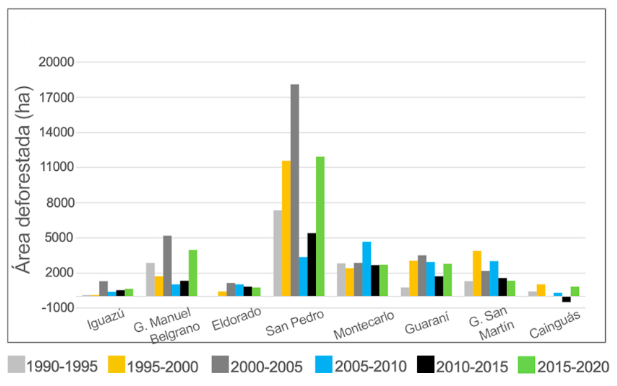
\includegraphics[width=0.95\textwidth]{img/perdida_corredor_verde.png}
      
      \vspace{0.2em}
      {\tiny Fuente: \href{https://sobrelatierra.agro.uba.ar/desmonte-sin-pausa-en-misiones-bosques-mas-chicos-y-fragmentados/}{Sobre La Tierra (FAUBA)}}
    \end{column}
  \end{columns}
  \note{
    La deforestación ha sido significativa: \num{130000} hectáreas perdidas en \num{30}
    años. Aunque hay mejoras recientes (\qty{18}{\percent} de reducción en 2025), la presión
    continúa principalmente por ocupaciones ilegales en parcelas pequeñas.
  }
\end{frame}

\begin{frame}{Fragmentacion del Habitat}
  \begin{alertblock}{Consecuencias}
    \begin{itemize}
      \item Poblaciones aisladas geneticamente
      \item Desplazamiento por areas no protegidas
      \item Conflictos con actividades humanas
      \item Atropellamientos en rutas \footnote{\tiny \url{https://www.vidasilvestre.org.ar/?26580/Atropellamiento-una-seria-amenaza-para-la-fauna-misionera}}
    \end{itemize}
  \end{alertblock}

  % TODO: Diagrama de fragmentacion
  \centering
  \fbox{\parbox{0.7\textwidth}{\centering\vspace{1.5cm}
      [Diagrama fragmentacion del habitat]
  \vspace{1.5cm}}}
  \note{
    La fragmentación aísla poblaciones, reduce la diversidad genética y obliga
    a los animales a cruzar zonas no protegidas, donde enfrentan riesgos
    adicionales como atropellamientos.
  }
\end{frame}

\begin{frame}{Caza Furtiva}
  \begin{columns}
    \begin{column}{0.55\textwidth}
      \textbf{Dos dimensiones:}
      \begin{enumerate}
        \item \textbf{Cultural/subsistencia:} Residentes locales
        \item \textbf{Economica/organizada:} Trafico de fauna
      \end{enumerate}

      \vspace{0.5em}
      \textbf{Zonas criticas:}
      \begin{itemize}
        \item Frontera con Brasil
        \item Reserva de Biosfera Yaboti
        \item Parques provinciales Pinalito, Urugua-i
      \end{itemize}

      \vspace{0.5em}
      \textbf{Especies afectadas:} Tapir, paca, corzuelas, tucanes, loros
    \end{column}
    \begin{column}{0.45\textwidth}
      % TODO: Imagen relacionada a caza furtiva
      \centering
      \fbox{\parbox{0.9\textwidth}{\centering\vspace{2cm}
          [Imagen problematica\\caza furtiva]
      \vspace{2cm}}}
    \end{column}
  \end{columns}
  \note{
    La caza furtiva tiene dos caras: la cultural/subsistencia de pobladores
    locales y el tráfico organizado. Las zonas fronterizas son especialmente
    críticas. Especies como el tapir y los loros son muy afectadas.
  }
\end{frame}

\begin{frame}{Intrusion en Areas Protegidas}
  \textbf{Actividades ilicitas frecuentes:}
  \begin{itemize}
    \item Pesca ilegal en cursos de agua
    \item Desmonte encubierto para expansion de cultivos
    \item Campamentos de caza con infraestructura permanente
    \item Extraccion de recursos naturales
  \end{itemize}

  \vspace{1em}
  \begin{alertblock}{Problema critico}
    Sin un sistema de \textbf{alerta temprana}, las intrusiones se descubren \textbf{a posteriori} durante patrullajes de rutina, cuando el dano ya fue perpetrado.
  \end{alertblock}
  \note{
    Sin alertas en tiempo real, las intrusiones se detectan tardíamente. Este
    es el problema central que nuestro proyecto busca resolver: transformar el
    monitoreo pasivo en vigilancia activa.
  }
\end{frame}

\section*{Contramedidas y Desafíos en Conservación}
\begin{frame}{Desafios de la Vigilancia}
  \textbf{\num{780000} hectareas} distribuidas en \textbf{\num{106}+ areas protegidas}

  \vspace{0.5em}
  \begin{description}
    \item[Extension:] Terreno accidentado, vegetacion densa, acceso limitado
    \item[Comunicaciones:] Sin cobertura celular en zonas interiores
    \item[Latencia:] Semanas/meses entre captura de evento y descubrimiento
    \item[Volumen:] Miles de imagenes requieren clasificacion manual
  \end{description}

  % TODO: Foto de terreno/vegetacion densa
  \centering
  \fbox{\parbox{0.5\textwidth}{\centering\vspace{1.2cm}
      [Foto vegetacion densa]
  \vspace{1.2cm}}}
  \note{
    \num{780000} hectáreas en más de \num{100} áreas protegidas. Sin cobertura celular,
    con terreno difícil y miles de imágenes que clasificar manualmente. Estos
    desafíos motivan nuestra propuesta tecnológica.
  }
\end{frame}

\begin{frame}{Contramedidas Tradicionales}
  \textbf{Métodos actuales de vigilancia:}
  \begin{itemize}
    \item Patrullajes de guardaparques (a pie o vehículo)
    \item Monitoreo por audio
    \item Drones y radares
    \item \textbf{Cámaras trampa pasivas} (el método más extendido)
  \end{itemize}
  \note{
    Para combatir estas amenazas, se utilizan diversas contramedidas. Los
    patrullajes son limitados por recursos. Se usan drones y monitoreo de
    audio, pero el método más extendido por su costo-beneficio son las
    cámaras trampa pasivas.
  }
\end{frame}

\begin{frame}{Uso de Cámaras Trampa}
  \begin{columns}
    \begin{column}{0.5\textwidth}
      \textbf{¿Cómo funcionan?}
      \begin{itemize}
        \item Se activan mediante sensores de movimiento (PIR).
        \item Capturan imágenes al detectar presencia (fauna o intrusos).
      \end{itemize}

      \vspace{0.5em}
      \textbf{Modalidades de operación:}
      \begin{itemize}
        \item \textbf{Pasivas:} Almacenan las imágenes en una tarjeta SD local (requiere recolección manual).
        \item \textbf{Activas (Comerciales):} Utilizan redes 3G/4G o conexiones satelitales para transmitir datos al instante.
      \end{itemize}
    \end{column}
    \begin{column}{0.5\textwidth}
      % TODO: Foto camara trampa
      \centering
      \fbox{\parbox{0.9\textwidth}{\centering\vspace{2cm}
          [Foto cámara trampa]
      \vspace{2cm}}}
    \end{column}
  \end{columns}
  \note{
    Las cámaras trampa son el método más utilizado. Se activan por movimiento y toman una foto. Existen dos modalidades: las pasivas que guardan la foto en una tarjeta SD, y las activas que la envían usando infraestructura de telecomunicaciones.
  }
\end{frame}

\begin{frame}{Limitaciones del Monitoreo Actual}
  \begin{block}{Cámaras Pasivas: El problema de la latencia}
    ¿Cuánto tiempo tarda entre que ocurre una intrusión y nos enteramos? \textbf{Mucho tiempo}. Pueden pasar semanas hasta recolectar la memoria SD. Para entonces, el daño ya está hecho.
  \end{block}

  \begin{block}{Cámaras Activas: Infraestructura y Costos}
    \begin{itemize}
      \item \textbf{Dependencia celular:} En la selva profunda la señal es inexistente.
      \item \textbf{Altos costos operativos:} Suscripciones mensuales o hardware satelital excesivamente caro.
      \item \textbf{Baja escalabilidad:} Económicamente inviable para despliegues masivos en grandes extensiones.
    \end{itemize}
  \end{block}
  \note{
    Las pasivas tienen una latencia inaceptable: la información llega tarde. Las activas resuelven la latencia pero dependen de infraestructura que no hay en la selva, además de ser muy caras e imposibles de escalar masivamente.
  }
\end{frame}

\section*{El Rol de la Tecnología en Conservación}
\begin{frame}{Aplicaciones de la IA en la Conservación}
  \textbf{La Inteligencia Artificial ofrece nuevas herramientas:}
  
  \vspace{0.5em}
  \begin{description}
    \item[AiCatcher:] Raspberry Pi + LoRa para inferencia en borde (Mallya, 2019) \footcite{mallya2019aicatcher}.
    \item[Microsoft WildLife:] Ecosistema de herramientas impulsadas por IA.
    \item[YOLO:] Algoritmos de detección de objetos en tiempo real.
    \item[MegaDetector:] Modelos pre-entrenados para detección de fauna.
  \end{description}
  \note{
    La IA está transformando la conservación. Proyectos como AiCatcher usan
    Raspberry Pi y LoRa, aunque con alto consumo. Microsoft tiene su
    iniciativa WildLife, y existen modelos robustos como YOLO y MegaDetector que automatizan la revisión de imágenes.
  }
\end{frame}

% ==============================================================================
% Sección 2: Objetivos (Nuestra Propuesta)
% ==============================================================================
\section{Objetivos}

\begin{frame}{Nuestra Propuesta}
  \begin{alertblock}{Solución}
    Diseño e implementación de un \textbf{Sistema de Monitoreo y Alerta Temprana basado en IA} para áreas protegidas.
  \end{alertblock}
  
  \vspace{1em}
  \textbf{Pilares del sistema:}
  \begin{itemize}
    \item \textbf{Barato y escalable} (hardware económico y open source)
    \item \textbf{Reducción del tiempo de respuesta} (de semanas a minutos)
    \item \textbf{Cobertura en zonas remotas} (red malla independiente)
    \item \textbf{Eliminación de ruido} (IA para evitar falsos positivos)
  \end{itemize}
  \note{
    Nuestra propuesta es un Sistema de Monitoreo y Alerta Temprana. Sus 4
    pilares son: que sea barato y escalable, que reduzca drásticamente la
    latencia, que funcione en zonas remotas sin celular, y que elimine los
    falsos positivos usando IA.
  }
\end{frame}

% \begin{frame}{Motivacion del Proyecto}
% \textbf{Transformar el paradigma:}

% \begin{center}
% Monitoreo \textbf{pasivo} $\longrightarrow$ Vigilancia \textbf{activa e inteligente}
% \end{center}

% \vspace{1em}
% \textbf{Un sistema que:}
% \begin{itemize}
% \item No solo capture imagenes, sino que las \textbf{transmita en tiempo real}
% \item Las \textbf{analice automaticamente} mediante IA
% \item Genere \textbf{alertas inmediatas} ante eventos de interes
% \item Sea \textbf{accesible y de bajo costo}
% \item Use \textbf{hardware economico} y \textbf{software de codigo abierto}
% \end{itemize}
% \note{
% Nuestra motivación: pasar del monitoreo pasivo (revisar fotos semanas
% después) a vigilancia activa con alertas inmediatas. Un sistema accesible,
% de bajo costo, con código abierto.
% }
% \end{frame}

% \begin{frame}{Oportunidad Tecnologica}
% \textbf{Convergencia de tres desarrollos:}

% \vspace{0.5em}
% \begin{block}{1. Microcontroladores de bajo costo}
% ESP32: WiFi, Bluetooth, bajo consumo. Costo: $<$ \qty{10}{\$} USD
% \end{block}

% \begin{block}{2. Redes mesh autoorganizadas}
% ESP-MESH-LITE: Extension de cobertura sin infraestructura celular
% \end{block}

% \begin{block}{3. IA para vision por computadora}
% SpeciesNet, MegaDetector: Modelos de codigo abierto para clasificacion automatica de fauna
% \end{block}
% \note{
% Tres tecnologías convergen: ESP32 a menos de \num{10} dólares con WiFi integrado,
% redes mesh que extienden cobertura sin infraestructura, y modelos de IA de
% código abierto como SpeciesNet.
% }
% \end{frame}

% \begin{frame}{Objetivo General}
% \begin{alertblock}{Objetivo}
% Demostrar la \textbf{viabilidad tecnica} de un sistema de monitoreo de \textbf{bajo costo} para areas protegidas, basado en:
% \begin{itemize}
% \item Nodos de camara con conectividad \textbf{mesh}
% \item Clasificacion automatica de imagenes mediante \textbf{IA}
% \end{itemize}
% \end{alertblock}

% \vspace{1em}
% \textbf{Reduccion del tiempo de procesamiento:}
% \begin{center}
% \textbf{Dias/semanas} $\longrightarrow$ \textbf{Minutos}
% \end{center}
% \note{
% El objetivo central es demostrar viabilidad técnica. No comercialización,
% sino prueba de concepto funcional. El cambio clave: reducir el tiempo de
% procesamiento de días a minutos.
% }
% \end{frame}

% \begin{frame}{Objetivos Especificos}
% \begin{enumerate}
% \item Disenar e implementar un \textbf{nodo de camara autonomo} basado en ESP32

% \item Desarrollar una \textbf{red mesh autoorganizada} con ESP-MESH-LITE

% \item Implementar un \textbf{servidor de procesamiento} con IA

% \item Integrar \textbf{SpeciesNet/MegaDetector} para clasificacion

% \item \textbf{Validar el funcionamiento} en condiciones reales
% \end{enumerate}
% \note{
% Cinco objetivos específicos que abarcan hardware, red, servidor, IA y
% validación. Cada uno corresponde a un componente del sistema que
% desarrollamos.
% }
% \end{frame}


% ==============================================================================
% Sección 3: Desarrollo (Arquitectura)
% ==============================================================================
\section{Desarrollo}

\begin{frame}{Vision General}
\centering
\includegraphics[width=0.95\textwidth]{bachelor-thesis/img/arquitecturaGeneralH.jpg}
\note{
Visión general del sistema: nodos de cámara capturan imágenes, las envían por
red mesh al nodo raíz, que las reenvía al servidor para procesamiento con IA
y notificación por Telegram.
}
\end{frame}

\begin{frame}{Nodo de Camara - Hardware}
\begin{columns}
\begin{column}{0.5\textwidth}
\textbf{Componentes:}
\begin{itemize}
  \item ESP32-CAM (AI-Thinker)
  \item Camara OV2640 (\num{2}~MP)
  \item Sensor PIR HC-SR501
  \item Buck converter LM2596
  \item Baterias 18650 (2S, \qty{7.4}{\volt})
\end{itemize}

\vspace{0.5em}
\textbf{Resolucion:} \num{640} x \num{480} (VGA)
\end{column}
\begin{column}{0.5\textwidth}
\centering

\includegraphics[width=0.9\textwidth]{bachelor-thesis/img/nodoEnsamblado.jpg}
\end{column}
\end{columns}
\note{
Hardware del nodo: ESP32-CAM de AI-Thinker con cámara OV2640, sensor PIR
HC-SR501, buck converter para alimentación desde baterías 18650. Resolución
VGA suficiente para clasificación.
}
\end{frame}

\begin{frame}{Diseno y Energia}

% Fila 1: Render / Esquematico horizontal
\centering
\includegraphics[width=0.85\textwidth]{bachelor-thesis/img/modelo3D.png}

\vspace{1em}

% Fila 2: Dos columnas
\begin{columns}
  \begin{column}{0.55\textwidth}
  \textbf{Autonomia (Baterias 18650 2S \qty{3500}{mAh}):}
  \begin{itemize}
  \item Capacidad util: $\sim$\qty{1400}{mAh} (corte a \qty{6.5}{V} por dropout LM2596)
  \item Autonomia medida (Relay): $\sim$\qty{5}{h}
  \end{itemize}
  \end{column}
  
  \begin{column}{0.45\textwidth}
  \textbf{Consumo Energetico (\unit{\milli\ampere}):}
  \begin{table}
  \centering
  \scriptsize
  \begin{tabular}{lc}
  \hline
  \textbf{Estado} & \textbf{Consumo} \\
  \hline
  Modo ULP (Leaf, Deep Sleep) & $\sim$\num{13} \\
  Promedio (Relay, Light Sleep) & $\sim$\num{180} \\
  Captura y envio & $\sim$\num{200} \\
  \hline
  \end{tabular}
  \end{table}
  \end{column}
\end{columns}
\note{
En el diseño físico protegimos los componentes con una carcasa 3D.
El aspecto clave es la energía: usamos baterías 18650 2S.
Como el LM2596 tiene una caída de voltaje, perdemos capacidad utilizable.
El nodo Leaf usa el coprocesador ULP en Deep Sleep consumiendo solo 13mA.
El nodo Relay debe mantener la red viva, consumiendo 180mA (5hs autonomía).
}
\end{frame}

\begin{frame}{Red Malla - El Concepto}
\textbf{¿Como sacamos la foto de la selva profunda?}

\vspace{0.5em}
\textbf{Protocolo: ESP-MESH-LITE}
\begin{itemize}
\item Solucion sobre WiFi $2.4$GHz (Modo SoftAP + Station)
\item Extiende el alcance sin depender de infraestructura celular
\item Comportamiento de router: el reenvio de paquetes de otros nodos ocurre transparentemente a nivel de red (IP)
\end{itemize}

\vspace{1em}
\begin{alertblock}{Flujo de Datos Transparente}
Cuando el PIR detecta movimiento, el nodo despierta y realiza una \textbf{peticion HTTP POST}. A partir de ahi, los nodos intermedios simplemente leen la direccion IP destino y enrutan los paquetes salto por salto hasta el servidor.
\end{alertblock}
\note{
Para sacar la foto de la selva usamos ESP-MESH-LITE. Un detalle clave a 
destacar: los nodos actúan literalmente como routers. La capa de
aplicación de cada nodo solo se encarga de originar su propia foto. Cuando un
nodo ``Relay'' recibe paquetes de otros nodos, los reenvía directamente
viendo la IP, sin involucrar a su capa de aplicación.
}
\end{frame}

\begin{frame}{Red Malla - Topologia y Roles}
\begin{columns}
\begin{column}{0.5\textwidth}
\textbf{Topologia de Arbol:}
\begin{itemize}
\item Multiples conexiones descendentes (SoftAP)
\item Una unica conexion ascendente (Station)
\end{itemize}

\vspace{0.5em}
\textbf{Roles (Trade-off de Energia):}
\begin{description}
\item[Leaf:] Nivel mas bajo. Deep Sleep + ULP. Ultra bajo consumo.
\item[Relay:] Nodo intermedio. Light Sleep para enrutar trafico.
\item[Root:] Unica puerta de enlace al Router. 100\% activo. Sin camara.
\end{description}
\end{column}
\begin{column}{0.5\textwidth}
\centering
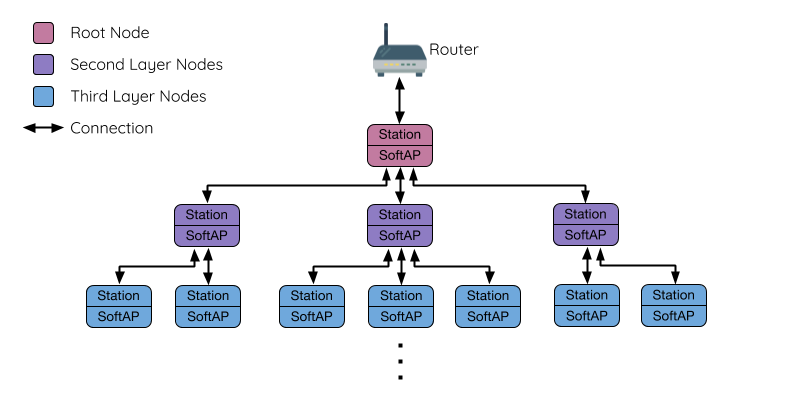
\includegraphics[width=0.95\textwidth]{img/mesh-tree-topology.png}
\end{column}
\end{columns}
\note{
La red tiene topología de árbol. Tenemos 3 roles con un fuerte trade-off
energético: El Leaf prioriza ahorro de batería (Deep sleep, sin enrutar).
El Relay sacrifica batería para extender la red (Light sleep).
El Root es el nodo raíz (un ESP32 sin cámara) que puentea a internet.
}
\end{frame}

\begin{frame}{Red Malla - Robustez (Self-Healing)}
\textbf{Auto-recuperacion ante fallos (Self-Healing):}

\vspace{0.5em}
\begin{itemize}
\item Si un nodo Relay se desconecta o queda sin bateria, los nodos hijos \textbf{re-escanean} el entorno y seleccionan un nuevo padre disponible, reparando la red en $< \qty{45}{s}$.
\item Prevencion de bucles (Loop Prevention) interna.
\end{itemize}

\vspace{0.5em}
\textbf{Seleccion automatica del Root Node:}
\begin{itemize}
\item Multiples nodos Root evaluan su senal \textbf{RSSI} respecto al Router.
\item El nodo con mejor senal asume el rol de Root y los demas se convierten en nodos secundarios. Evita cuellos de botella.
\end{itemize}
\note{
La robustez es crítica en la selva. MESH-LITE nos da self-healing: si un
nodo intermedio se cae, los hijos buscan automáticamente otro padre.
Además, la elección del nodo raíz es dinámica basada en la mejor señal
RSSI con el router principal.
}
\end{frame}




\begin{frame}{Servidor de Aplicacion}
\centering
\scalebox{0.6}{
  \begin{tikzpicture}[
      scale=0.8,
      font=\sffamily,
      >=Latex,
      node distance=14mm and 22mm,
      service/.style={
        draw=black!70,
        rounded corners=2pt,
        fill=blue!3,
        minimum width=22mm,
        minimum height=9mm,
        align=center,
        line width=0.9pt
      },
      volume/.style={
        draw=black!70,
        cylinder,
        shape border rotate=90,
        aspect=0.28,
        minimum height=9mm,
        minimum width=18mm,
        align=center,
        fill={rgb,255:red,253;green,250;blue,228},
        draw={rgb,255:red,134;green,122;blue,34},
        line width=0.9pt
      },
      bindmount/.style={
        draw=black!70,
        diamond,
        aspect=2,
        inner xsep=2pt,
        inner ysep=1.5pt,
        fill={rgb,255:red,253;green,250;blue,228},
        draw={rgb,255:red,134;green,122;blue,34},
        line width=0.9pt,
        font=\ttfamily\footnotesize,
        align=center
      },
      app/.style={-{Latex[length=2.2mm,width=1.6mm]}, draw=black!70, line width=0.95pt},
      mount/.style={Latex-Latex, draw=black!65, dashed, line width=0.95pt}
    ]

    % Service nodes
    \node[service] (web) {web (Django)};
    \node[service, left=of web] (bot) {bot (Telegram)};
    \node[service, right=of web] (db) {db (PostgreSQL)};
    \node[service, below=of web] (speciesnet) {speciesnet (Inferencia)};

    % Volume and bind mount nodes
    \node[bindmount, above left=12mm and 12mm of web] (Vstatic) {./static};
    \node[bindmount, above=of web] (Vmonitorstatic) {./monitor/static};
    \node[volume, left=24mm of speciesnet] (Vmediavolume) {media\_volume};
    \node[volume, below=of speciesnet] (Vspeciesnetcache) {speciesnet\_cache};
    \node[volume, below=of db] (Vdbdata) {db\_data};

    % Inter-service communication
    \draw[app] (bot) -- (web);
    \draw[app] (web) -- (db);
    \draw[app] (web) -- (speciesnet);

    % Volume mounts / bind mounts
    \draw[mount] (Vstatic) -- (web);
    \draw[mount] (Vmonitorstatic) -- (web);
    \draw[mount] (Vmediavolume) -- (web);
    \draw[mount] (Vmediavolume) -- (bot);
    \draw[mount] (Vspeciesnetcache) -- (speciesnet);
    \draw[mount] (Vmediavolume) -- (speciesnet);
    \draw[mount] (Vdbdata) -- (db);

  \end{tikzpicture}
}
\note{
Servidor containerizado con Docker Compose: Django para backend,
SpeciesNet para inferencia con LitServe, PostgreSQL para datos, bot de
Telegram para notificaciones. Fácil de desplegar.
}
\end{frame}

\begin{frame}{Servicio de Deteccion (SpeciesNet)}
  \begin{columns}
    \begin{column}{0.5\textwidth}
      \textbf{Pipeline de procesamiento:}
      \begin{enumerate}
        \item \textbf{Deteccion:} MegaDetector (YOLOv5) identifica regiones de interes (animal, persona, vehiculo).
        \item \textbf{Clasificacion:} Modelos SpeciesNet analizan recortes y predicen familia, genero y especie.
        \item \textbf{Anotacion:} Genera copia con bounding boxes.
      \end{enumerate}
      \vspace{0.5em}
      \textbf{API REST:} Endpoint \texttt{/predict} expuesto mediante LitServe.
    \end{column}
    \begin{column}{0.5\textwidth}
      \centering
      \scalebox{0.5}{
        \begin{tikzpicture}[
            node distance=1.0cm and 1.5cm,
            box/.style={rectangle, draw, rounded corners, fill=blue!10, text width=3.8cm, text centered, minimum height=1.2cm, font=\sffamily\small},
            io/.style={trapezium, trapezium left angle=70, trapezium right angle=110, draw, fill=green!10, text width=3.2cm, text centered, minimum height=1.0cm, font=\sffamily\small},
            process/.style={rectangle, draw, fill=orange!10, text width=3.8cm, text centered, minimum height=1.2cm, font=\sffamily\small},
            arrow/.style={thick, -Latex}
          ]
  
          % Nodos
          \node (request) [io] {HTTP POST \texttt{/predict}};
          \node (read) [process, below=of request] {Lectura de Imagen};
          \node (detect) [box, below=of read] {Deteccion\\(MegaDetector)};
          \node (classify) [box, below=of detect] {Clasificacion\\(SpeciesNet)};
          \node (draw) [process, below=of classify] {Anotacion de Imagen};
          \node (save) [process, below=of draw] {Guardado de Imagen};
          \node (response) [io, below=of save] {Respuesta JSON};
  
          % Conexiones
          \draw [arrow] (request) -- (read);
          \draw [arrow] (read) -- (detect);
          \draw [arrow] (detect) -- node[anchor=east, font=\scriptsize] {Recortes} (classify);
          \draw [arrow] (classify) -- node[anchor=east, font=\scriptsize] {Clases} (draw);
          \draw [arrow] (draw) -- (save);
          \draw [arrow] (save) -- (response);
          \draw [arrow] (detect.east) -- ++(1.0,0) |- (draw.east);
  
        \end{tikzpicture}
      }
    \end{column}
  \end{columns}
\note{
Pipeline de 3 fases dentro del contenedor SpeciesNet: MegaDetector detecta
y localiza objetos, clasificador taxonómico identifica especies, y se
genera una imagen anotada. Todo expuesto via API REST con LitServe.
}
\end{frame}

\begin{frame}{Logica de Umbrales de Deteccion}
\textbf{Tres niveles de decision para enviar alertas:}

\vspace{0.5em}
\begin{description}
\item[HIGH = 0{,}80:] Confianza $>$ \qty{80}{\percent} $\rightarrow$ alerta \textbf{inmediata}, sin importar clasificacion
\item[MID = 0{,}50:] Confianza entre \qty{50}{\percent} y \qty{80}{\percent} y clasificador dice ``vacio'' $\rightarrow$ alerta igualmente (posible animal pequeno)
\item[LOW = 0{,}30:] Confianza $<$ \qty{30}{\percent} y clasificador ``vacio'' $\rightarrow$ se \textbf{descarta} (probable falso positivo del PIR)
\end{description}

\vspace{0.5em}
\begin{alertblock}{Politica}
Sesgo hacia la \textbf{sensibilidad}: ante la duda, se transmite la imagen y se delega la decision al operador humano.
\end{alertblock}
\note{
Tres umbrales configurables: HIGH (80\%) envía siempre, MID (50\%) envía
si el clasificador dice vacío (posible animal pequeño), LOW (30\%) descarta.
Política conservadora: preferimos falsos positivos a perder eventos reales.
}
\end{frame}

\begin{frame}{Sistema de Alertas}
\begin{columns}
\begin{column}{0.5\textwidth}
\textbf{Bot de Telegram}

\vspace{0.5em}
Cada notificacion incluye:
\begin{itemize}
  \item Imagen original
  \item Imagen anotada (bounding boxes)
  \item Cantidad y confianza de detecciones
  \item Top 5 clasificaciones taxonomicas
\end{itemize}

\vspace{1em}
\textbf{Human-in-the-loop:}
\begin{itemize}
  \item Teclados inline para \textbf{corregir} clasificaciones
  \item Genera datos para futuro \textit{fine-tuning}
\end{itemize}
\end{column}
\begin{column}{0.5\textwidth}
\centering
\includegraphics[width=0.7\textwidth]{bachelor-thesis/img/notificacionTelegramLab.png}
\end{column}
\end{columns}
\note{
Bot de Telegram envía imagen original + anotada + detecciones + top 5
clasificaciones. 
(Oral: Mencionar brevemente que tiene comandos básicos como /start para registro y /last para pedir la última foto).
Incluye retroalimentación interactiva (Human-in-the-loop): el usuario puede
corregir clasificaciones con teclados inline, generando datos etiquetados
para futuro fine-tuning del modelo.
}
\end{frame}

% Limitaciones Conocidas movido a la Sección 5

% ==============================================================================
% Sección 4: Resultados
% ==============================================================================
\section{Resultados}

\begin{frame}{Pruebas de Campo}
\begin{columns}
\begin{column}{0.5\textwidth}
\textbf{Lugar:} Jardin botanico

\vspace{0.3em}
\textbf{Condiciones:}
\begin{itemize}
\item Duracion: \qty{5}{h} de operacion continua
\item 3 nodos desplegados
\item Distancia entre nodos: \qty{15}{m}
\item Condiciones climaticas: soleado
\end{itemize}

\vspace{0.3em}
\textbf{Detecciones exitosas:}
\begin{itemize}
\item Personas (intrusos)
\item Vehiculos
\item Aves silvestres (conf. 0.74-0.90)
\item Gato domestico (conf. 0.96)
\end{itemize}
\end{column}
\begin{column}{0.5\textwidth}
  \centering
  \begin{figure}
    \begin{subfigure}[b]{0.9\textwidth}
      \centering
      \includegraphics[height=3.3cm]{bachelor-thesis/img/nodoCampo1.jpg}
      \caption{Despliegue en Campo}
    \end{subfigure}
    \vfill
    \begin{subfigure}[b]{0.9\textwidth}
      \centering
      \includegraphics[height=3.3cm]{bachelor-thesis/img/capturaIntrusoProcesada.png}
      \caption{Deteccion de Intruso}
    \end{subfigure}
  \end{figure}
\end{column}
\end{columns}
\note{
Arrancamos los resultados demostrando que el sistema funciona en la realidad. 
Pruebas de campo en jardín botánico: 5 horas, soleado, 3 nodos a 15 m
entre sí. Detecciones exitosas de personas, vehículos, aves silvestres
(confianza 0.74-0.90) y gato doméstico (0.96). Falsas activaciones por
movimiento de vegetación fueron filtradas por la lógica de umbrales.
}
\end{frame}

\begin{frame}{Live Demo del Sistema}
  \centering
  \fbox{\parbox{0.8\textwidth}{\centering\vspace{3cm}
      [Espacio para demostración en vivo o video]\\
      (Activación de cámara $\rightarrow$ Mesh $\rightarrow$ Telegram)
  \vspace{3cm}}}
  \note{
    Aquí realizamos la demostración en vivo. Activamos una cámara,
    la petición viaja por la red mesh al servidor local, procesa la imagen
    y llega la notificación al bot de Telegram frente a todos.
  }
\end{frame}

\begin{frame}{Resultados - Red Mesh}
\begin{table}
\centering
\begin{tabular}{lc}
\hline
\textbf{Metrica}               & \textbf{Valor} \\
\hline
Latencia LAN (\qty{12.9}{\kilo\byte})  & $\sim$\qty{463}{ms}   \\
Ciclo completo nodo (LAN)     & $\sim$\qty{1.27}{s}   \\
Latencia campo (hotspot)      & \qtyrange{20}{60}{s} (prom. \qty{40}{s}) \\
Distancia max (linea de vista) & \qtyrange{15}{18}{m}  \\
Distancia max (vegetacion)     & $\sim$\qty{12}{m}     \\
Distancia max (interior)       & $\sim$\qty{10}{m}     \\
\hline
\end{tabular}
\end{table}
\note{
Métricas de red: en LAN, transmisión HTTP de 463 ms para 12.9 KB, ciclo
completo de 1.27 s. En campo con hotspot celular (cobertura deficiente),
latencia promedio de 40 s. Distancia máxima: 15-18 m en línea de vista,
12 m con vegetación, 10 m en interior.
}
\end{frame}

\begin{frame}{Resultados - Deteccion}
\begin{columns}
\begin{column}{0.5\textwidth}
\textbf{Deteccion binaria} (\num{94} imagenes):
\begin{table}
\normalsize
\renewcommand{\arraystretch}{1.3}
\begin{tabular}{lc}
\hline
\textbf{Metrica} & \textbf{Valor} \\
\hline
Exactitud   & \qty{77.7}{\percent}  \\
Precision   & \qty{78.9}{\percent}  \\
Recall      & \qty{69.8}{\percent}  \\
\hline
\end{tabular}
\end{table}

\vspace{0.3em}
\textbf{Recall por clase:}
\begin{itemize}
  \item Animales: \qty{52.9}{\percent}
  \item Personas: \qty{77.3}{\percent}
  \item Vehiculos: \qty{100}{\percent}
\end{itemize}
\end{column}
\begin{column}{0.55\textwidth}
  \centering
  \begin{figure}
    \begin{subfigure}[b]{0.48\textwidth}
      \centering
      \includegraphics[width=\textwidth]{bachelor-thesis/img/confusion_matrix_binary.png}
      \caption{Binaria}
    \end{subfigure}
    \hfill
    \begin{subfigure}[b]{0.48\textwidth}
      \centering
      \includegraphics[width=\textwidth]{bachelor-thesis/img/confusion_matrix.png}
      \caption{Multiclase}
    \end{subfigure}
  \end{figure}
\end{column}
\end{columns}
\note{
Resultados sobre 94 imágenes de campo. Exactitud general 77.7\%.
Animales es la clase más difícil (52.9\% recall) por fauna pequeña que
se confunde con el fondo. Personas 77.3\%. El enfoque Human-in-the-loop
compensa estos errores y genera datos para fine-tuning.
}
\end{frame}

% El frame de Consumo Energético fue movido a la Sección 3 (Diseño y Energía)

% 
% \begin{frame}{Pruebas de Laboratorio}
% \textbf{Validaciones realizadas:}
% 
% \begin{itemize}
% \item Captura de imagen: inicializacion, calidad, tamano
% \item Sensor PIR: distancia, tiempo de respuesta, falsas activaciones
% \item Transmision mesh: conexion, latencia, perdida de paquetes
% \item Clasificacion: deteccion de animales/personas/vehiculos
% \item Alertas: recepcion en Telegram, contenido correcto
% \end{itemize}
% \note{
% Pruebas de laboratorio cubrieron cada componente: captura de imagen, sensor
% PIR, transmisión mesh, clasificación con IA, y recepción de alertas en
% Telegram.
% }
% \end{frame}
% 
% \begin{frame}{Resultados - Captura de Imagen}
% % TODO: Ejemplo imagen capturada
% \centering
% \fbox{\parbox{0.6\textwidth}{\centering\vspace{2cm}
% [Ejemplo imagen capturada 640x480]
% \vspace{2cm}}}
% 
% \begin{itemize}
% \item Resolucion: 640x480 (VGA)
% \item Formato: JPEG comprimido
% \item Tamano tipico: \qtyrange{30}{35}{\kilo\byte}
% \item Ciclo completo (deteccion $\rightarrow$ envio): $\sim$\qty{1.27}{s} en LAN
% \end{itemize}
% \note{
% Resultados de captura: resolución VGA suficiente para clasificación.
% Imágenes JPEG de 30-35 KB. Ciclo completo desde detección PIR hasta
% confirmación de envío: 1.27 segundos en red local.
% }
% \end{frame}

% ==============================================================================
% Sección 5: Conclusiones
% ==============================================================================
\section{Conclusiones}

\begin{frame}{Logros Alcanzados}
\begin{itemize}
\item[$\checkmark$] Sistema completo de monitoreo con \textbf{hardware de bajo costo}
\item[$\checkmark$] Reduccion de tiempo de procesamiento: \textbf{dias $\rightarrow$ minutos}
\item[$\checkmark$] Red mesh funcional con \textbf{ESP-MESH-LITE} (roles Leaf/Relay/Root)
\item[$\checkmark$] Integracion exitosa de \textbf{SpeciesNet/MegaDetector}
\item[$\checkmark$] Sistema de alertas via \textbf{Telegram} con retroalimentacion \textit{Human-in-the-loop}
\item[$\checkmark$] Carcasa imprimible en 3D (disponible en Printables)
\item[$\checkmark$] \textbf{Codigo abierto} disponible en GitHub
\end{itemize}
\note{
Resumen de logros: sistema completo funcionando, reducción de tiempo de
días a minutos, red mesh estable con ESP-MESH-LITE y roles diferenciados,
IA integrada, alertas por Telegram con Human-in-the-loop, carcasa 3D,
todo código abierto.
}
\end{frame}

% Aportes del Trabajo movido a Anexos

\begin{frame}{Comparacion con Objetivos}
\begin{table}
\centering
\small
\begin{tabular}{lc}
\hline
\textbf{Objetivo} & \textbf{Resultado} \\
\hline
Deteccion de fauna, personas y vehiculos & Accuracy \qty{77.7}{\percent} (\num{94} imgs) \\
Latencia de respuesta & $\sim$\qty{40}{s} (campo) / \qty{1.27}{s} (LAN) \\
Cobertura mesh & \qtyrange{15}{18}{m} (linea de vista) \\
Autonomia (Relay) & $\sim$\qty{5}{h} medidas \\
Consumo Leaf (ULP) & $\sim$\qty{13}{mA} \\
\hline
\end{tabular}
\end{table}

\vspace{0.3em}
\begin{alertblock}{Conclusion}
Se demostro la \textbf{viabilidad tecnica} del sistema propuesto. Mejora de \textbf{ordenes de magnitud} respecto a camaras trampa convencionales.
\end{alertblock}
\note{
Comparación objetivo vs. resultado. Detección funcional con 77.7\% accuracy.
Latencia de 40 s en campo (vs. semanas en cámaras convencionales).
Cobertura de 15-18 m suficiente para despliegue en cadena. Autonomía de
5 h en Relay, consumo Leaf de apenas 13 mA.
}
\end{frame}

\begin{frame}{Limitaciones Conocidas}
\begin{description}
\item[Operacion diurna:] Lente con filtro IR, sin vision nocturna
\item[Sensor PIR:] Optimizado para humanos, puede no detectar fauna pequena
\item[Resolucion:] VGA (640$\times$480), limitada por el balance entre calidad JPEG y tiempo de transmision
\item[Consumo:] WiFi consume mas que camaras trampa comerciales optimizadas
\item[Gestion de energia:] Nodos intermedios (Relay) deben mantener conectividad mesh permanente, limitando su autonomia
\end{description}

\vspace{0.5em}
\begin{block}{Nota sobre ``tiempo real''}
No es tiempo real deterministico (milisegundos), sino \textbf{operativo}: de dias/semanas a \textbf{minutos}.
\end{block}
\note{
Transparencia sobre limitaciones: sin visión nocturna, PIR domótico,
resolución VGA limitada por el balance compresión/transmisión.
Nodos Relay deben mantener la red activa (Light Sleep), lo que reduce
autonomía. Tiempo real significa minutos, no milisegundos.
}
\end{frame}

\begin{frame}{Trabajos Futuros}
\begin{description}
\item[Vision nocturna:] Camaras con capacidad infrarroja
\item[Conectividad largo alcance:] LoRa, \num{4}G/LTE, satelital para zonas remotas
\item[Nodo repetidor dedicado:] Nodo sin camara que mantenga la red mesh, permitiendo Deep Sleep puro en nodos camara
\item[Optimizacion energetica:] Paneles solares, reguladores mas eficientes
\item[Actualizacion OTA:] Firmware inalambrico sin recoleccion fisica de nodos
\item[Optimizacion de alcance:] Antenas de mayor ganancia, calibracion RSSI, mayor compresion
\item[Procesamiento en borde:] TinyML en nodos de camara
\item[Modelos especificos:] Fine-tuning para fauna del Bosque Atlantico
\end{description}
\note{
Líneas futuras: visión nocturna, conectividad largo alcance, nodo
repetidor dedicado para mejorar autonomía, OTA updates, optimización de
alcance entre nodos, TinyML, fine-tuning con datos del Human-in-the-loop.
}
\end{frame}

% Recomendaciones y Repositorios movidos a Anexos

\begin{frame}{Agradecimientos}
\begin{itemize}
\item A nuestras familias por el apoyo incondicional
\item Al Dr. Ing. Sergio Moya por su guía y dedicación como tutor
\item A la Facultad de Ingeniería de la UNaM
\item A los docentes que contribuyeron a nuestra formación
\item A nuestros compañeros de carrera
\end{itemize}

\vspace{1em}
\centering
\textit{¡Gracias a todos!}
\note{
Agradecer especialmente a las familias, al tutor Dr. Sergio Moya, a la
Facultad de Ingeniería, docentes y compañeros. Este proyecto no hubiera
sido posible sin su apoyo.
}
\end{frame}

\begin{frame}[standout]
¿Preguntas?
\end{frame}

\begin{frame}[allowframebreaks]{Referencias}
\printbibliography[heading=none]
\end{frame}

% ==============================================================================
% Slides de Backup
% ==============================================================================
\appendix

\begin{frame}{Esquemático del Hardware}
\centering
\includegraphics[width=0.9\textwidth]{bachelor-thesis/img/kicad-capstone-project.pdf}
\note{
Backup: Esquemático completo del nodo cámara diseñado en KiCad. Muestra
conexiones entre ESP32-CAM, sensor PIR, buck converter y baterías.
}
\end{frame}

\begin{frame}{Planos de la Carcasa}
\begin{columns}
  \begin{column}{0.5\textwidth}
    \centering
    \includegraphics[height=0.75\textheight]{bachelor-thesis/img/ESP3-CAM Drawing Main Case.pdf}
  \end{column}
  \begin{column}{0.5\textwidth}
    \centering
    \includegraphics[height=0.75\textheight]{bachelor-thesis/img/ESP3-CAM Drawing Base.pdf}
  \end{column}
\end{columns}
\note{
Backup: Planos 2D de la carcasa con dimensiones exactas. Permite
fabricación con otros métodos además de impresión 3D.
}
\end{frame}

\begin{frame}{Análisis Económico}
\begin{columns}
\begin{column}{0.5\textwidth}
\textbf{Inversión inicial:} \$20,530 USD

\vspace{0.5em}
\textbf{Modelo de negocio:}
\begin{itemize}
\item Cobro por instalación
\item Suscripción mensual (\$50 USD)
\end{itemize}

\vspace{0.5em}
\textbf{Mercado objetivo:}
\begin{itemize}
\item 116 reservas naturales
\item 10,800+ EAPs con bosques
\end{itemize}
\end{column}
\begin{column}{0.5\textwidth}
\textbf{Indicadores:}
\begin{itemize}
\item VAN: \qty{7517.55}{\$} USD
\item TIR: \qty{25}{\percent}
\item TREMA: \qty{15}{\percent}
\item Recupero: Ano \num{4}
\end{itemize}

\vspace{0.5em}
\textbf{Conclusion:}\\
Proyecto \textbf{economicamente viable}
\end{column}
\end{columns}
\note{
Backup: Análisis económico. Inversión inicial de \qty{20530}{\$} USD. Modelo de
suscripción mensual. VAN positivo, TIR del \qty{25}{\percent} supera TREMA del \qty{15}{\percent}.
Recupero en año \num{4}. Proyecto económicamente viable.
}
\end{frame}

\begin{frame}{Sensibilidad Económica}
\centering
\scalebox{0.7}{
  \begin{tikzpicture}
    \begin{axis}[
        name=left axis,
        width=0.8\textwidth,
        height=5cm,
        xlabel={Suscripciones anuales},
        ylabel={VAN (USD)},
        axis y line*=left,
        grid=major,
        xmin=18, xmax=32,
        ymin=-8000, ymax=12000,
        xtick={20,22,24,26,28,30},
        scaled ticks=false,
        mark size=3pt,
        legend style={at={(0.02,0.98)}, anchor=north west},
      ]
      \addplot[blue, thick, mark=*] coordinates {
        (20, -6373.04)
        (22, -2900.39)
        (24, 572.26)
        (26, 4044.90)
        (28, 7517.55)
        (30, 10990.20)
      };
      \addplot[gray, dashed, thick] coordinates {(18,0) (32,0)};
      \legend{VAN, VAN = 0}
    \end{axis}
    \begin{axis}[
        width=0.8\textwidth,
        height=5cm,
        axis y line*=right,
        axis x line=none,
        ylabel={TIR (\%)},
        ylabel near ticks,
        xmin=18, xmax=32,
        ymin=-100, ymax=50,
        mark size=3pt,
        legend style={at={(0.98,0.02)}, anchor=south east},
      ]
      \addplot[red, thick, mark=square*] coordinates {
        (20, -80)
        (22, -35)
        (24, -11)
        (26, 8)
        (28, 25)
        (30, 41)
      };
      \addplot[orange, dashed, thick] coordinates {(18,15) (32,15)};
      \legend{TIR, TREMA (15\%)}
    \end{axis}
  \end{tikzpicture}
}

\begin{itemize}
  \scriptsize
  \item Punto de equilibrio: \num{24} suscripciones/ano
  \item Precio minimo viable: \qty{40}{\$} USD/mes
\end{itemize}
\note{
Backup: Análisis de sensibilidad. Punto de equilibrio en \num{24} suscripciones
anuales. Precio mínimo viable de \qty{40}{\$} USD/mes antes de que el proyecto deje
de ser rentable.
}
\end{frame}

\begin{frame}{Alcance del Proyecto}
\begin{columns}
\begin{column}{0.5\textwidth}
\textbf{Dentro del alcance:}
\begin{itemize}
  \item Nodos ESP32-CAM + sensor PIR
  \item Red mesh funcional
  \item Servidor de recepcion y clasificacion
  \item Bot de Telegram para alertas
  \item Pruebas en laboratorio y campo
\end{itemize}
\end{column}
\begin{column}{0.5\textwidth}
\textbf{Fuera del alcance:}
\begin{itemize}
  \item Despliegue en selva densa
  \item Carcasas con grado IP
  \item Entrenamiento de modelos especificos
  \item Certificacion comercial
\end{itemize}
\end{column}
\end{columns}
\note{
Definimos claramente qué sí y qué no incluye el proyecto. Prototipo
funcional para pruebas, no producto comercial. Sin despliegue en selva
real ni carcasas industriales.
}
\end{frame}

\begin{frame}{Nodo de Camara - Firmware}
\textbf{Desarrollado con ESP-IDF + ESP-MESH-LITE}

\vspace{0.5em}
\textbf{Funcionalidades compartidas:}
\begin{itemize}
\item Inicializacion de sistema (NVS, event loop, interfaces de red)
\item Configuracion de red ESP-MESH-LITE en modo AP-STA
\item Captura y compresion JPEG con camara OV2640
\item Almacenamiento en microSD (respaldo)
\item Peticion \textbf{HTTP POST} estandar al servidor
\end{itemize}

\vspace{0.3em}
\textbf{Diferenciacion por rol:}
\begin{description}
\item[Relay:] Interrupcion GPIO para PIR. Light Sleep + Modem Sleep.
\item[Leaf:] Coprocesador ULP (polling cada \qty{100}{ms}). Deep Sleep total.
\end{description}
\note{
Firmware con ESP-IDF + ESP-MESH-LITE. Ambos roles comparten la
inicialización y captura. La diferencia clave: Relay usa interrupción
GPIO y Light Sleep, Leaf usa el coprocesador ULP con polling cada 100ms
y Deep Sleep completo. Cada nodo hace HTTP POST estándar, no hay Mwifi.
}
\end{frame}

\begin{frame}{Carcasa Impresa en 3D}
\begin{columns}
\begin{column}{0.5\textwidth}
\textbf{Diseno basado en modelo CC \num{4.0}}

\vspace{0.5em}
\textbf{Caracteristicas:}
\begin{itemize}
  \item Material: PLA
  \item Apertura para lente
  \item Domo para sensor PIR
  \item Espacio para buck converter
  \item Acceso a tarjeta SD
  \item Puntos de montaje
\end{itemize}

\vspace{0.5em}
\textit{Disponible en Printables}
\end{column}
\begin{column}{0.5\textwidth}
\centering
\includegraphics[width=0.85\textwidth]{bachelor-thesis/img/carcasaNodo.jpg}
\end{column}
\end{columns}
\note{
Carcasa impresa en 3D basada en diseño CC 4.0. PLA, aperturas para lente y
PIR, espacio para electrónica, acceso a SD, puntos de montaje. Disponible
en Printables para que cualquiera pueda fabricarla.
}
\end{frame}

\begin{frame}{Nodo Raiz}
\begin{columns}
\begin{column}{0.55\textwidth}
\textbf{Hardware:} ESP32 DevKit V1 (sin camara)

\vspace{0.5em}
\textbf{Rol:} Puerta de enlace Mesh $\leftrightarrow$ Internet

\vspace{0.5em}
\textbf{Funciones:}
\begin{itemize}
  \item Nivel 1 de la red ESP-MESH-LITE
  \item Punto de acceso permanente (SoftAP)
  \item Enrutamiento transparente (NAT, DHCP)
  \item Conexion WiFi STA a router
  \item Reporte periodico de estado (cada \qty{10}{s})
\end{itemize}
\end{column}
\begin{column}{0.45\textwidth}
\centering
\includegraphics[width=0.95\textwidth]{bachelor-thesis/img/Diagramas Tesis-Diagra de Flujo nodo Root.jpg}
\end{column}
\end{columns}
\note{
Nodo raíz: ESP32 DevKit sin cámara, opera exclusivamente en Nivel 1.
Mantiene SoftAP permanente, enrutamiento transparente con NAT y DHCP.
Reporta estado de la red cada 10 segundos. No usa modos de bajo consumo.
}
\end{frame}

\begin{frame}{Configuracion de Pruebas}
\begin{columns}
\begin{column}{0.5\textwidth}
\textbf{Hardware:}
\begin{itemize}
\item 3 nodos de camara (ESP32-CAM)
\item 1 nodo raiz (ESP32 DevKit)
\item Baterias 18650 (2S, \qty{3500}{mAh})
\item Router WiFi domestico
\end{itemize}
\end{column}
\begin{column}{0.5\textwidth}
\textbf{Software:}
\begin{itemize}
\item ESP-IDF v5 + ESP-MESH-LITE
\item Docker containers
\item SpeciesNet + LitServe
\item PostgreSQL 15
\end{itemize}
\end{column}
\end{columns}

\centering
\includegraphics[width=0.65\textwidth]{bachelor-thesis/img/lab1.png}
\note{
Configuración de pruebas: 3 nodos cámara ESP32-CAM, 1 nodo raíz ESP32
DevKit, baterías 18650 2S de 3500 mAh, router doméstico. Software:
ESP-IDF v5 + ESP-MESH-LITE, Docker, SpeciesNet con LitServe, PostgreSQL 15.
Inferencia exclusivamente en CPU.
}
\end{frame}

\begin{frame}{Aportes del Trabajo}
\begin{block}{Arquitectura integrada}
Captura distribuida + transmision mesh + procesamiento IA centralizado
\end{block}

\begin{block}{Prototipo de bajo costo}
Componentes comerciales economicos + disenos 3D listos para fabricacion
\end{block}

\begin{block}{Integracion de SpeciesNet}
Pipeline de clasificacion taxonomica en tiempo operativo
\end{block}

\begin{block}{Codigo abierto}
\num{3} repositorios publicos en GitHub
\end{block}
\note{
Backup: Cuatro aportes principales: arquitectura integrada end-to-end, prototipo
replicable de bajo costo, primera integración de SpeciesNet en tiempo
operativo, y todo disponible como código abierto en 3 repositorios.
}
\end{frame}

\begin{frame}{Recomendaciones}
\begin{enumerate}
\item \textbf{Ubicaciones:} Considerar distancia entre nodos y obstaculos
\item \textbf{Proteccion:} Usar PETG/ASA para despliegues permanentes
\item \textbf{Baterias:} Dimensionar segun frecuencia de activaciones
\item \textbf{Sensor PIR:} Evaluar alternativas para fauna pequena
\item \textbf{Monitoreo:} Implementar seguimiento de estado de nodos
\end{enumerate}
\note{
Backup: Recomendaciones prácticas para implementadores.
}
\end{frame}

\begin{frame}{Repositorios}
\small
\begin{description}
\item[Firmware nodos:] \url{github.com/GabyDs/trapcam_mesh}
\item[Servidor aplicacion:] \url{github.com/fabcontigiani/server-capstone-project}
\item[Servidor inferencia:] \url{github.com/fabcontigiani/wildlife-detection-capstone-project}
\end{description}

\vspace{1em}
\textbf{Modelo 3D carcasa:} Disponible en Printables
\note{
Backup: Todo el código disponible en GitHub.
}
\end{frame}

\end{document}
